\chapter*{Introduction}\addcontentsline{toc}{chapter}{Introduction}


Black holes, paradoxically, power some of the brightest objects in the sky.  They strip gas off neighbouring stars and give rise to the x-ray binaries seen throughout the galaxy.  They swell to a billion times the mass of the sun and power active galactic nuclei, outshining galaxies and casting spotlights through intergalactic space.  They may even give rise to gamma-ray bursts, the brightest explosions ever observed which can be seen across the universe.

Strictly speaking, of course, black holes do not radiate themselves, at least not enough to be of astrophysical interest.  Rather accreting gas, falling deep into the black hole's gravitational potential, is able to reach extreme temperatures and radiate a great deal of energy before ultimately falling behind the black hole's event horizon.  The power source behind x-ray binaries, active galactic nuclei, and possibly gamma-ray bursts is an \emph{accretion disk}: a thin gaseous flow slowly spiraling into the black hole, trading gravitational potential energy for orbital velocity and heat.  The hot gas produces a spectrum of emission from the infrared to the x-ray, and in extreme cases even neutrinos.

These systems all show a rich variety of temporal and spectroscopic behaviour.  Black hole x-ray binaries undergo state changes between steady disk-dominated thermal emission and violent outbursts accompanied by non-thermal hard x-rays.  Active galactic nuclei (AGN) display stochastic, noisy optical light curves, non-thermal x-rays, and occasionally large collimated jets.  Gamma-ray bursts (GRBs) are brief flashes of gamma-rays followed by a long afterglow of x-ray, optical, and radio emission.  Although connected with the deaths of massive stars, the GRB central engine is still unknown.  Leading candidates include accretion onto a newly-formed black hole or spin-down of a magnetar during stellar core collapse \citep{Duncan92, Woosley93, Usov94, MacFadyen99, Metzger11}.

Most modeling of accretion disks is still based on the steady state Shakura-Sunyaev $\alpha$-disk, and its relativistic extension due to Novikov and Thorne (NT) \citep{ShakuraSunyaev, Novikov73}.  It is remarkable, and a testament to the authors, that this analytic model has held up so well over fifty years.  \fig{lmcx3spec} shows the x-ray spectrum of x-ray binary LMC X-3 with a fit to the NT model (from \citealt{Steiner14}).  The NT model with a small non-thermal component gives a very good fit to the observed spectrum.

\begin{figure}
\begin{center}
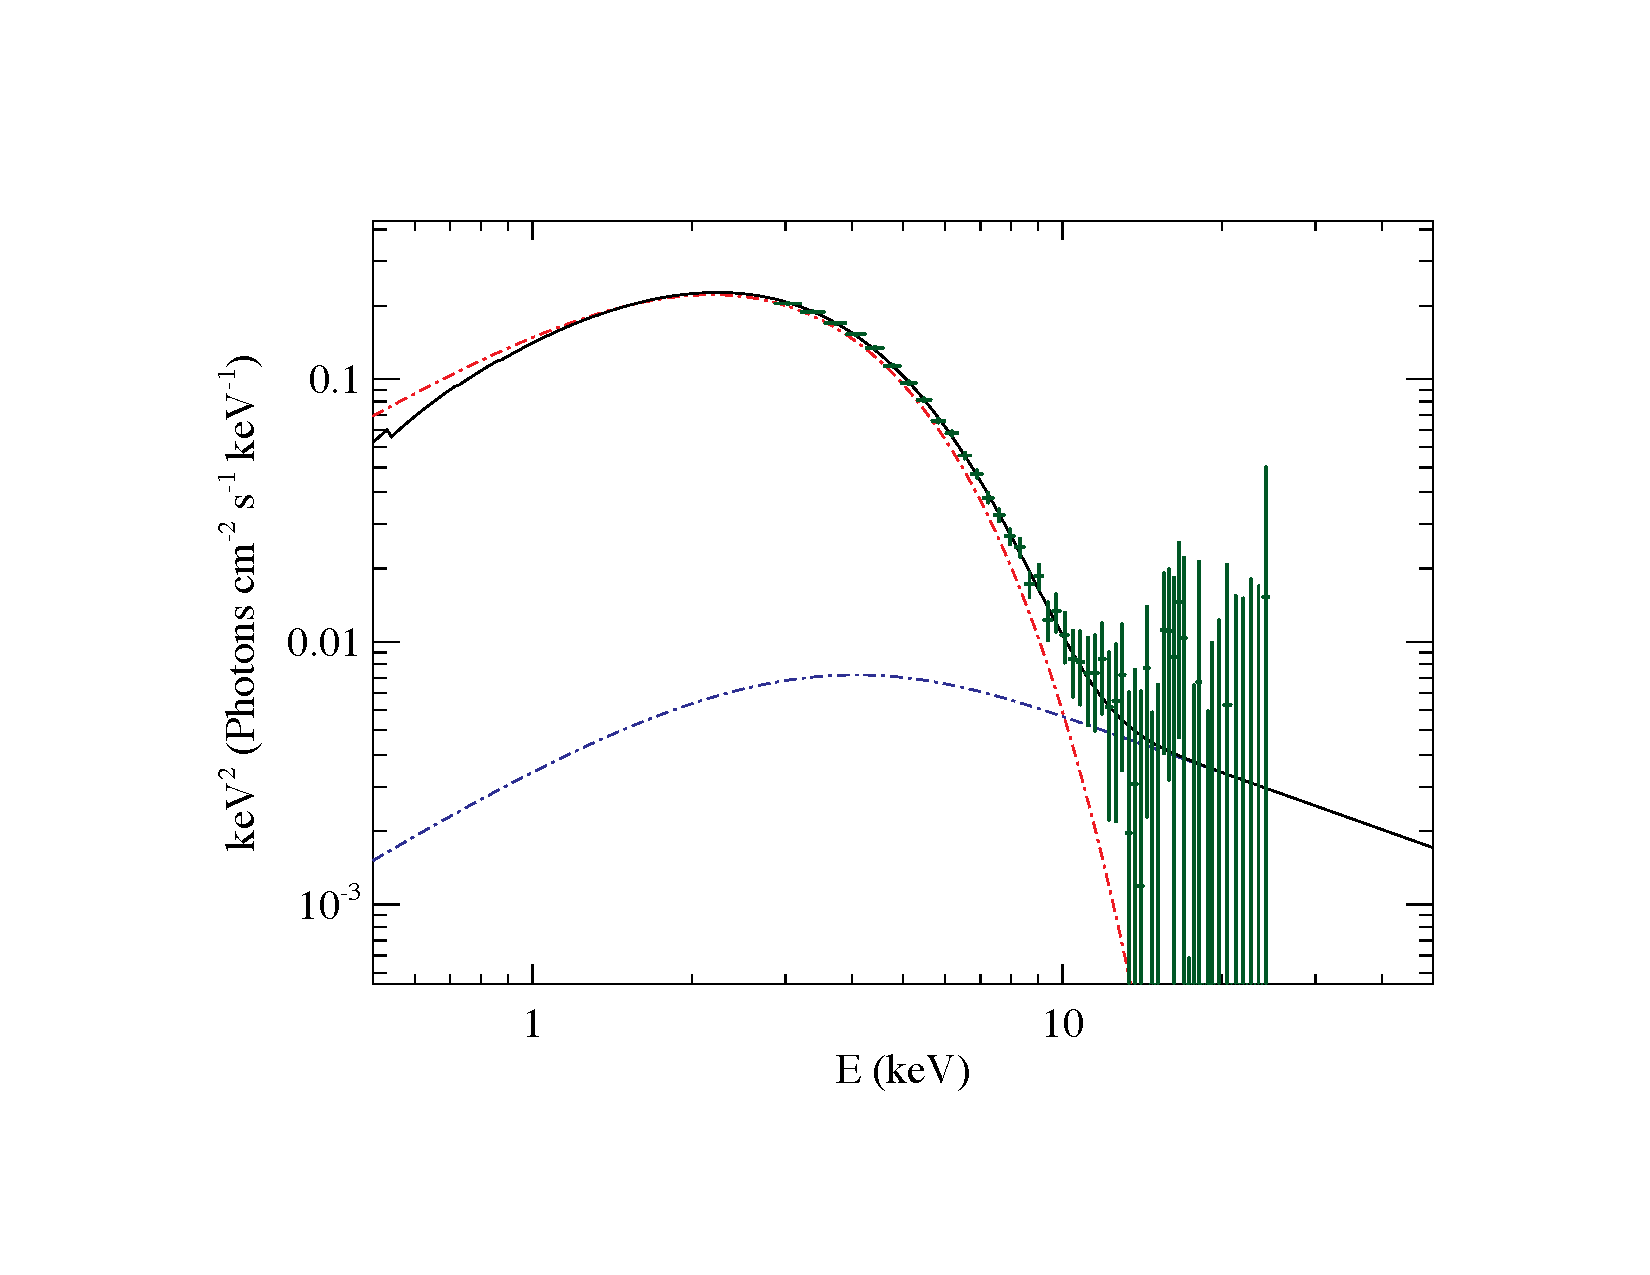
\includegraphics[width=0.6\textwidth]{figures/lmcx3spec.pdf}
\end{center}
\caption{The x-ray spectrum of black hole x-ray binary LMC X-3.  Rossi X-ray Timing Explorer (RXTE) data in green, Novikov--Thorne model fit in red dash-dotted, non-thermal component in blue dash-dotted, and full model in black.  The Novikov-Thorne model fits the thermal component very well. Figure from \cite{Steiner14}. \figlabel{lmcx3spec}}
\end{figure}

The NT model has two shortcomings: it explicitly assumes a steady state and it introduces an ad-hoc viscosity, the $\alpha$-prescription, to transport angular momentum and allow the disk to accrete.  The details of the angular momentum transport mechanism in real disks is still unknown.  The most likely candidate is magnetic stresses built up from the magneto-rotational instability (MRI) \citep{Balbus91}.  Other mechanisms include hydrodynamic Reynolds stresses, gravito-turbulence, and radiation pressure from the inner disk.  Each one of these mechanisms is time dependent, non-axisymmetric, and relies on non-linear processes in the gas flow which cannot be captured by a simple analytic model.

A system generating much interest is the accreting black hole binary.  It is known that galaxies which have undergone major mergers must at some point host two supermassive black holes, and by scattering with stars these black holes must migrate to the inner parsec of the galaxy.  Dubbed the ``final parsec problem,'' it is unknown what happens past this point, whether the black holes continue to orbit or eventually undergo a merger due to interactions with nearby gas, stars, or other black holes.  Recently candidate AGN hosting two black holes have been identified based on periodic modulations of their optical and infrared emission \citep{Graham15B, Charisi16}.  The best candidate, PG1302, whose light curve is shown in the left panel of \fig{SMBHB}, has a proposed period of only 5.7 years \citep{Graham15A}.  However, these candidates are in tension with recent null results from Pulsar Timing Arrays (PTAs), shown in the right panel of \fig{SMBHB}, which put an upper limit on the total number of such systems \citep{NanogravLimits, Sesana17}.   To resolve this tension better models of the emission from these systems are required.  Accreting black hole binaries are intrinsically time-dependent and asymmetric, limiting the utility of standard analytic models.  

\begin{figure}
\begin{center}
\begin{tabular}{cc}
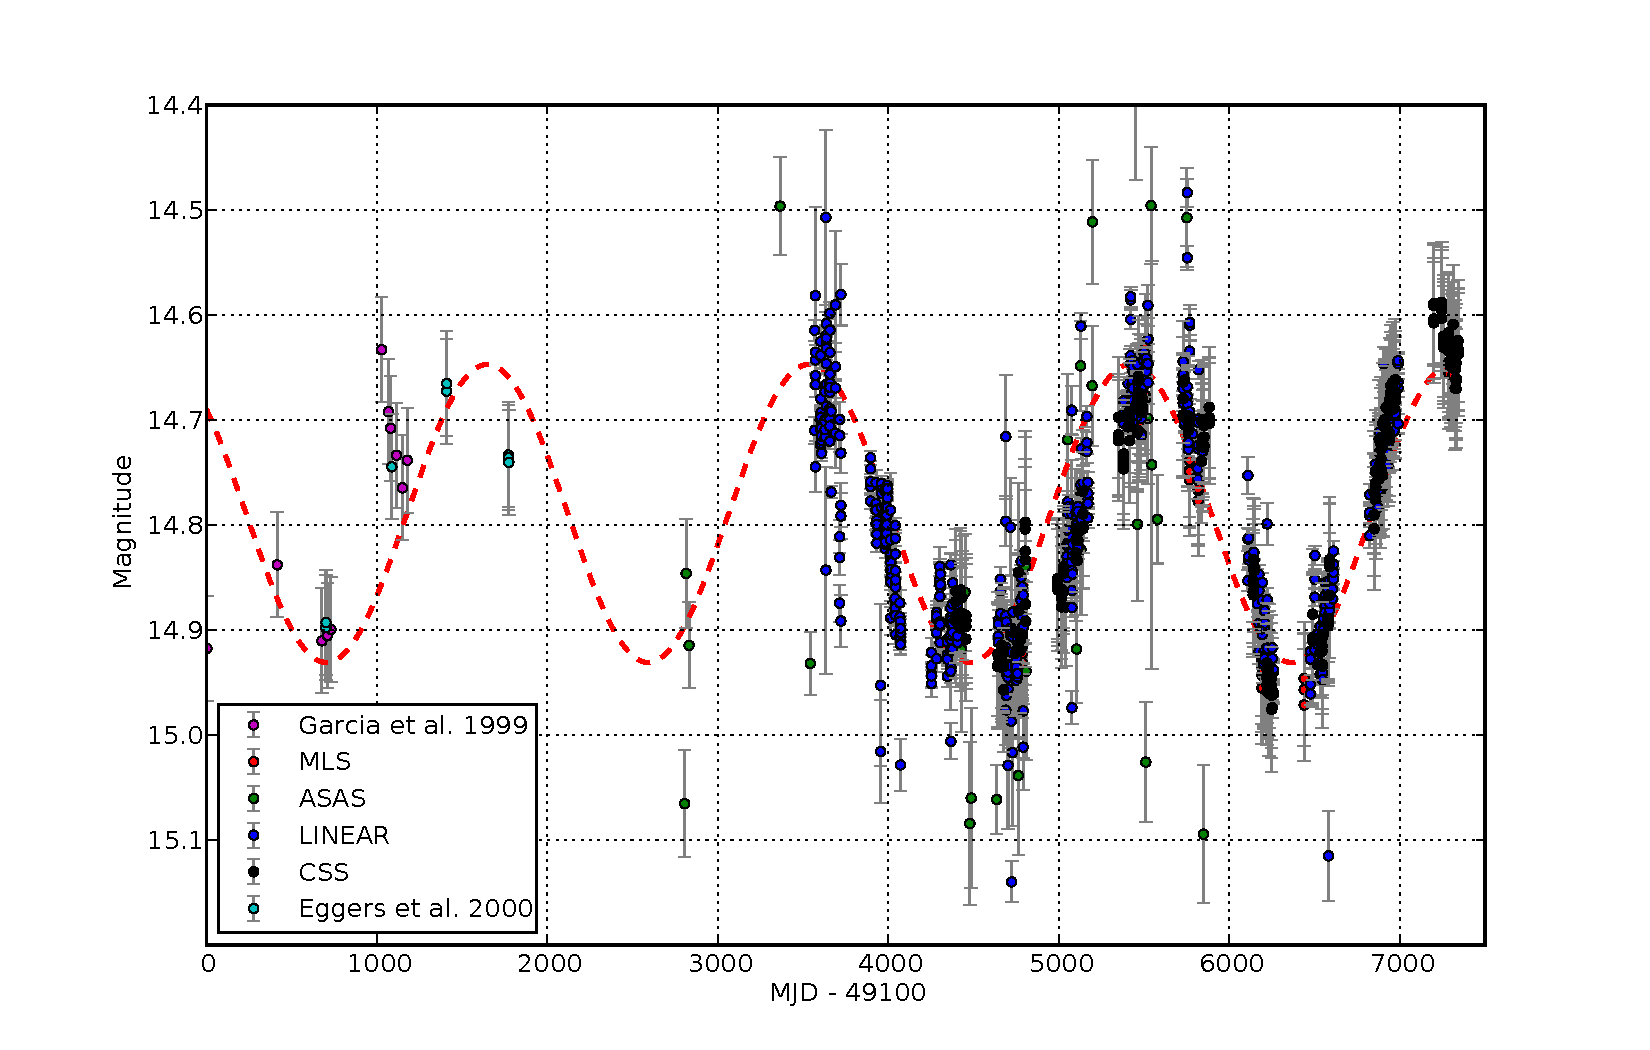
\includegraphics[width=0.45\textwidth]{figures/pg1302.pdf} & 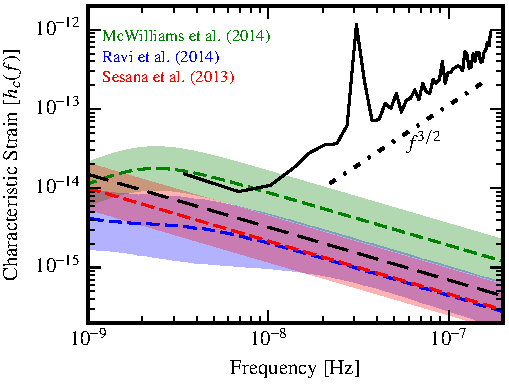
\includegraphics[width=0.4\textwidth]{figures/nanograv.pdf}
\end{tabular}
\end{center}
\caption{\emph{Left:} The optical light curve of quasar PG 1302-102.  A periodic variability with a period of 5.7 years may indicate the presence of a black hole binary in this system. From \cite{Graham15A}. \emph{Right:} Limits on the isotropic stochastic gravitational wave background from the Nanograv 9-year analysis.  The lack of observed gravitational waves is in tension with the number of candidate supermassive black hole binaries.  From \cite{NanogravLimits}. \figlabel{SMBHB}}
\end{figure}

The non-linear dynamics of the accretion mechanism and the time-dependence of target objects leave numerical simulation as the best tool to understand the details of black hole accretion.  In \chap{numerics} we present \grdisco, a three dimensional moving mesh general relativistic magnetohydrodynamics (GRMHD) code designed specifically to tackle black hole accretion disks.  This code is an extension of \disco, a Newtonian magnetohydrodynamics (MHD) code \citep{Duffell16}.  The moving mesh allows \disco\ to take much larger time steps than equivalent fixed grid codes while also virtually eliminating the advection errors which can accumulate after integrating a solution over many orbits.  \grdisco\ includes a relativistic $\alpha$-prescription to compare with steady state models and a microphysics module to enable study of disks with realistic equations of state.  The magnetic fields are evolved with a sophisticated constrained transport algorithm introduced in \cite{Duffell16}, preserving the divergence constraint to high precision and ensuring accurate evolution.  This allows \discogr\ to move away from the $\alpha$ prescription and consider long time-scale evolution of realistic black hole accretion disks.  

\chap{minidisk} presents the first use case for \grdisco: a study of the accretion dynamics in \emph{minidisks}.  Minidisks are accretion disks around the individual black holes in circumbinary black hole accretion (see Figure \ref{minidisk:fig:domain}).  They are the sources of the brightest emission in these systems and are nearest the black holes: necessitating a detailed relativistic treatment.  Zooming in on an individual minidisk we find spiral shockwaves, excited by tidal forces of the binary companion, provide for efficient angular momentum transport and drive accretion.  The effective $\al$ for these shocks is a few $\times 10^{-2}$.  Ray traced images provide for accurate spectra off these disks.  While broadly similar to the NT spectrum we see a high energy excess corresponding to shock dissipation near the innermost stable orbit of the black hole.  These calculations are relevant for any accretion disk in a binary system, both supermassive black hole binaries and stellar mass x-ray binaries.  

\chap{scalefit} presents an important application where numerical simulations are able to completely characterize a system and be compared to real data.  Although the GRB central engine is still unknown, the GRB afterglow is a very well-understood phenomenon: a relativistic blast wave producing synchrotron emission propagating through the circumburst medium.  We present a study of GRB afterglow light curves, with the ultimate aim of constraining the central engine properties.  Our model, \scalefit, utilizes a bank of template light curves calculated from ray-traced high resolution relativistic hydrodynamic simulations.  Scaling relations allow us to keep the template bank small while still covering the entire afterglow parameter space.  We ran this model on 226 \swiftXRT\ light curves, about one third of all GRB afterglow detected between 2005 and 2012.  We, for the first time, are able to measure the viewing angle of the jet, finding a median $\theta_{obs} \sim 0.6 \theta_{jet}$.  This has vast consequences for the central engine, as off-axis viewing can lower the required central engine energy output by a factor of four.  This puts the GRB energy within the range of magnetar models as well as black holes.

The aim of this thesis is to present a series of attempts to study black hole accretion by means of numerical simulations.  \chap{numerics} is methodological, introducing \grdisco, a new GRMHD code which should be able to simulate these systems with unprecedented accuracy.  The development of this code is ongoing, once completed the work in this chapter will be submitted for publication.  \chap{minidisk} uses \grdisco\ in a detailed study of minidisks in binary black hole systems.  The numerical treatment reveals the importance of an accretion mechanism that has to this point been ignored in these systems: spiral shockwaves excited by the binary companion.  This chapter has been published in The Astrophysical Journal as \cite{Ryan17}.  \chap{scalefit} presents a different use case altogether, identifying a phenomena that can be completely characterized by numerical simulation and using these simulations to construct a model that can be directly compared to data.  This approach gives us valuable information about GRBs, and demonstrates the role numerical simulation can play in observation as well as theory.  This chapter was published in The Astrophysical Journal as \cite{Ryan15}.  A companion paper using the same technique has been published as \cite*{Zhang15}.

